
\appendix
\section{Appendix}

\subsection{Robustness}
\label{sec:robust}

\begin{figure}[H]
	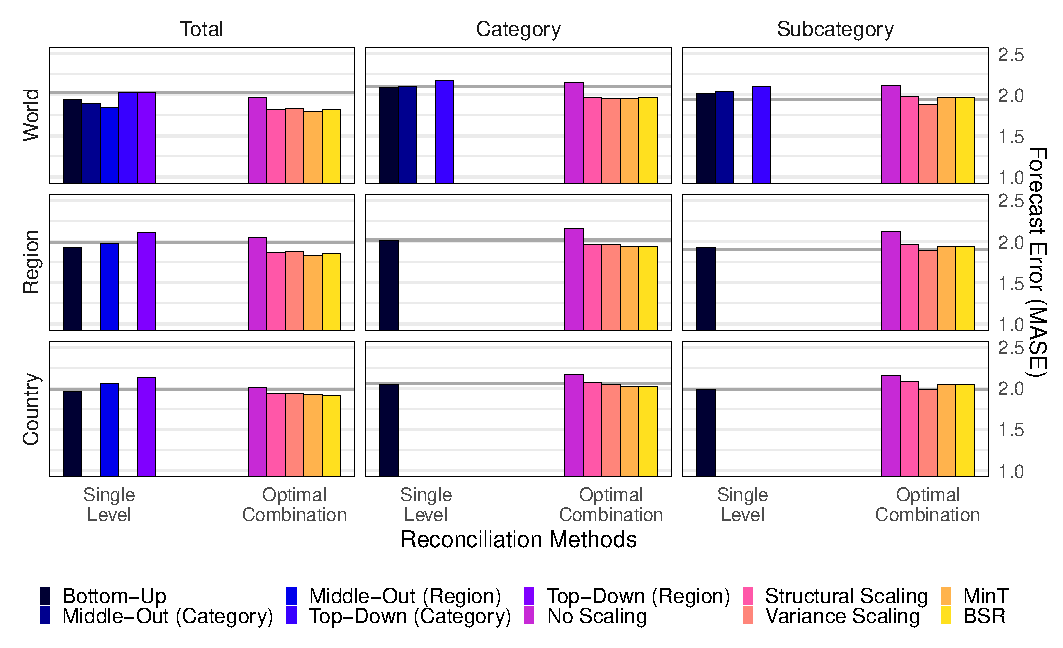
\includegraphics[width=\textwidth]{fig/fig_eval_mase}
	\caption[Forecast Errors of Reconciliation Methods]{\textbf{Forecast Errors of Reconciliation Methods (MASE).} \textit{Lower bars indicate better forecasts. Horizontal lines show the mean absolute scaled error of unreconciled predictions. Average of all forecast horizons.}}\label{fig:mase}
\end{figure}

\begin{figure}[H]
	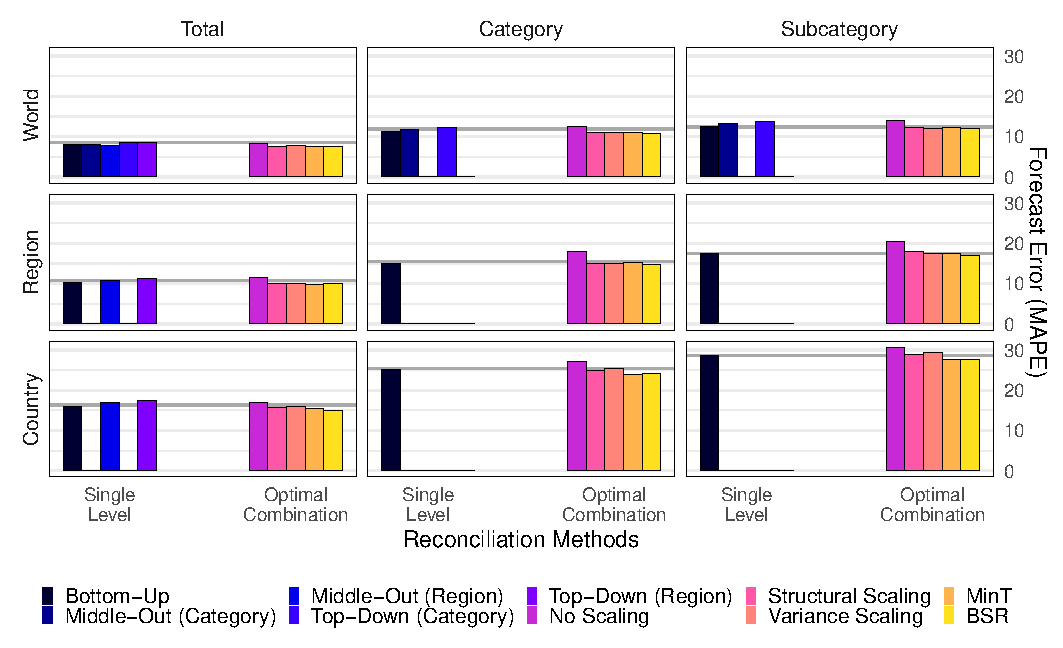
\includegraphics[width=\textwidth]{fig/fig_eval_mape}
	\caption[Forecast Errors of Reconciliation Methods]{\textbf{Forecast Errors of Reconciliation Methods (MAPE).} \textit{Lower bars indicate better forecasts. Horizontal lines show the mean absolute percentage error of unreconciled predictions. Average of all forecast horizons.}}\label{fig:mape}
\end{figure}

\begin{figure}[H]
	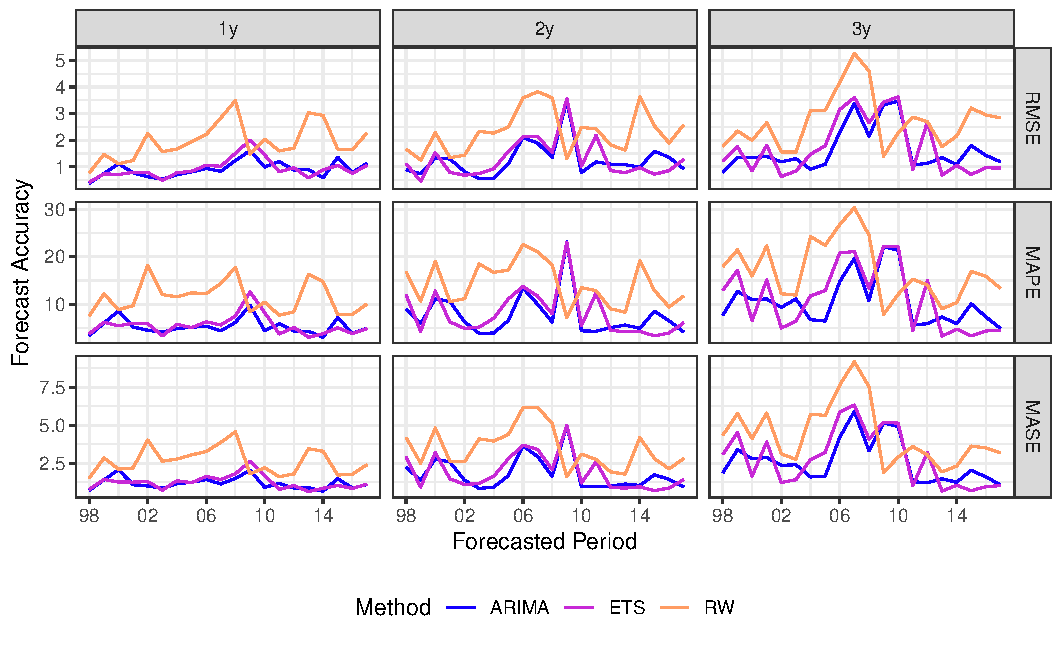
\includegraphics[width=\textwidth]{fig/fig_eval_methods_top}
	\caption{Accuracy of Forecasting Methods at the Top Level}
\end{figure}

\begin{figure}[H]
	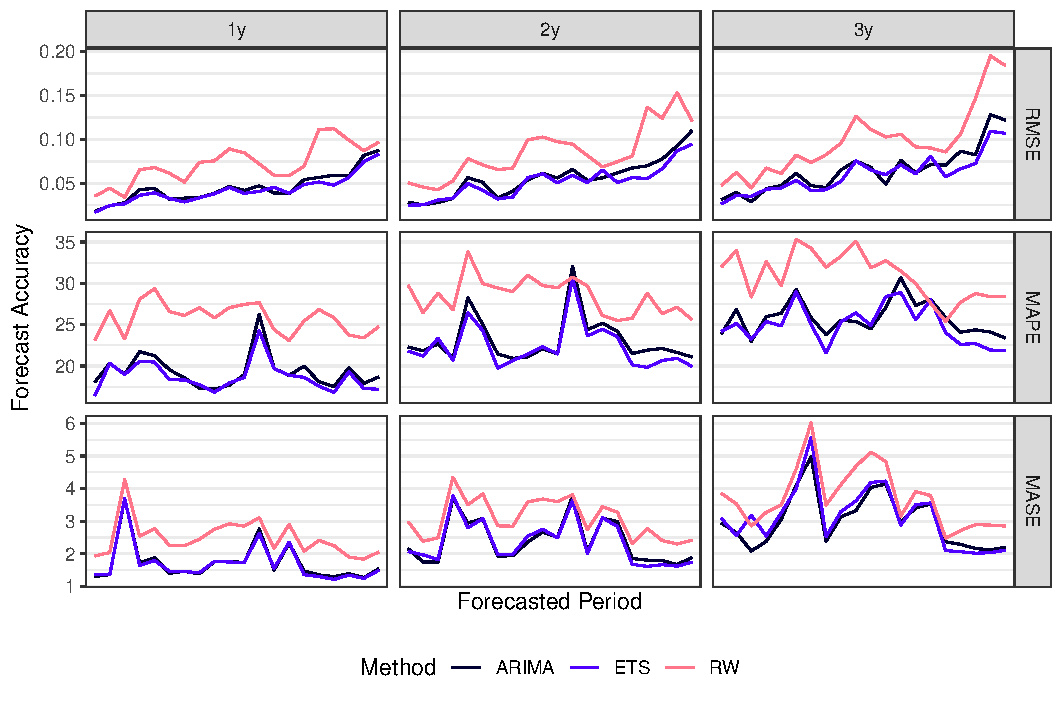
\includegraphics[width=\textwidth]{fig/fig_eval_methods_bottom}
	\caption{Accuracy of Forecasting Methods at the Bottom Level}
\end{figure}


\subsection{Data}
\label{sec:data}
The data is compiled by the Swiss Federal Customs Administration\footnote{\url{https://www.ezv.admin.ch/ezv/en/home/topics/swiss-foreign-trade-statistics.html}}.\\

\begin{small}
\begin{longtable}{p{1.5cm}p{12.8cm}}
\caption{Description of Categorical Hierarchy}\\
\toprule
\normalsize{No.} & \normalsize{Description}\\
\midrule
\endfirsthead
\multicolumn{2}{@{}l}{\ldots continued}\\
\toprule
\endhead
\bottomrule
\multicolumn{2}{r@{}}{continued \ldots}\\
\endfoot
\bottomrule
\endlastfoot
	01	&	Forestry and agricultural products, fisheries	\\
\enskip	01.1	&	Food, beverages and tobacco	\\
\enskip	01.2	&	Feeding stuffs for animals	\\
\enskip	01.3	&	Live animals	\\
\enskip	01.4	&	Horticultural products	\\
\enskip	01.5	&	Forestry products (not firewood)	\\
\enskip	01.6	&	Products for commercial/industrial further processing such as oils, fats, starches, plants and vegetable parts, etc.	\\
\midrule
	02	&	Energy source	\\
\enskip	02.1	&	Solid combustibles	\\
\enskip	02.2	&	Petroleum and distillates	\\
\enskip	02.3	&	Gas	\\
\enskip	02.4	&	Electrical energy	\\
\midrule
	03	&	Textiles, clothing, shoes	\\
\enskip	03.1	&	Textiles	\\
\enskip	03.2	&	Articles of apparel and clothing	\\
\enskip	03.3	&	Shoes, parts and accessories	\\
\midrule
	04	&	Paper, articles of paper and and products of the printing industry	\\
\enskip	04.1	&	Basic materials for paper production, such as cellulose and cellulose fibre and paper and carton waste	\\
\enskip	04.2	&	Paper and carton in rolls, strips or sheets	\\
\enskip	04.3	&	Goods from paper or carton	\\
\enskip	04.4	&	Products of the printing industry	\\
\midrule
	05	&	Leather, rubber, plastics	\\
\enskip	05.1	&	Leather	\\
\enskip	05.2	&	Rubber	\\
\enskip	05.3	&	Plastics	\\
\midrule
	06	&	Products of the chemical and pharmaceutical industry	\\
\enskip	06.1	&	Chemical raw materials, basic materials and unformed plastics	\\
\enskip	06.2	&	Chemical end products, vitamins, diagnostic products, including active substances	\\
\midrule
	07	&	Stones and earth	\\
\enskip	07.1	&	Mineral raw materials and basic products	\\
\enskip	07.2	&	Goods from stone and cement	\\
\enskip	07.3	&	Ceramic wares	\\
\enskip	07.4	&	Glass	\\
\midrule
	08	&	Metals	\\
\enskip	08.1	&	Iron and steel	\\
\enskip	08.2	&	Non-ferrous metals	\\
\enskip	08.3	&	Metal goods	\\
\midrule
	09	&	Machines, appliances, electronics	\\
\enskip	09.1	&	Industrial machinery	\\
\enskip	09.2	&	Agricultural machines	\\
\enskip	09.3	&	Household appliances	\\
\enskip	09.4	&	Office machines	\\
\enskip	09.5	&	Electrical and electronic industry appliances and devices	\\
\enskip	09.6	&	Military equipment	\\
\midrule
	10	&	Vehicles	\\
\enskip	10.1	&	Road vehicles	\\
\enskip	10.2	&	Railed vehicles	\\
\enskip	10.3	&	Air- and spacecraft	\\
\enskip	10.4	&	Watercraft	\\
\midrule
	11	&	Precision instruments, clocks and watches and jewellery	\\
\enskip	11.1	&	Precision instruments and equipment	\\
\enskip	11.2	&	Watches	\\
\enskip	11.3	&	Jewellery and household goods made from precious metals	\\
\midrule
	12	&	Various goods such as music instruments, home furnishings, toys, sports equipment, etc.	\\
\enskip	12.1	&	Exposed film	\\
\enskip	12.2	&	Music instruments	\\
\enskip	12.3	&	Home furnishings	\\
\enskip	12.4	&	Toys and sports equipment	\\
\enskip	12.5	&	Stationery goods	\\
\enskip	12.6	&	Various goods such as umbrellas, neon signs, festive articles, brushes, lighters, pipes, etc.	\\
\midrule
	13	&	Precious metals, precious and semi-precious stones	\\
\enskip	13.1	&	Precious and semi-precious stones	\\
\enskip	13.2	&	Precious metals (including gold and silver bars from 1.1.2012)	\\
\midrule
	14	&	Works of art and antiques	\\
\enskip	14.1	&	Works of art	\\
\enskip	14.2	&	Antiques and collectors' items	\\
\end{longtable}
\end{small}

\clearpage

\begin{small}
\begin{longtable}{p{0.5cm}p{9cm}p{2cm}p{2cm}}
		\caption{Description of Geographical Hierarchy}\\
		\toprule
Country	&	&	valid from	&	valid to	\\
		\midrule
		\endfirsthead
		\multicolumn{4}{@{}l}{\ldots continued}\\
		\toprule
		\endhead
		\bottomrule
		\multicolumn{4}{r@{}}{continued \ldots}\\
		\endfoot
		\bottomrule
		\endlastfoot
\multicolumn{3}{l}{Europe}	&	\\
DE	&	Germany	&	01/1988	&	-	\\

FR	&	France	&	01/1988	&	-	\\

IT	&	Italy	&	01/1988	&	-	\\

NL	&	Netherlands	&	01/1988	&	-	\\

BE	&	Belgium-Luxembourg	&	01/1988	&	12/1998	\\

BE	&	Belgium	&	01/1999	&	-	\\

LU	&	Luxembourg	&	01/1999	&	-	\\

AT	&	Austria	&	01/1988	&	-	\\

GB	&	United Kingdom	&	01/1988	&	-	\\

DK	&	Denmark	&	01/1988	&	-	\\

NO	&	Norway	&	01/1988	&	-	\\

SE	&	Sweden	&	01/1988	&	-	\\

PT	&	Portugal	&	01/1988	&	-	\\

FI	&	Finland	&	01/1988	&	-	\\

HR	&	Croatia, Republic of	&	02/1992	&	-	\\

SI	&	Slovenia	&	02/1992	&	-	\\

BA	&	Bosnia and Herzegovina	&	05/1992	&	-	\\

MK	&	North Macedonia	&	05/1992	&	-	\\

ME	&	Montenegro	&	05/1992	&	12/1996	\\

ME	&	Montenegro	&	01/2007	&	-	\\

XM	&	Montenegro	&	01/2006	&	12/2006	\\

SQ	&	Serbia	&	05/1992	&	12/1996	\\

RS	&	Serbia	&	01/2007	&	-	\\

XS	&	Serbia	&	01/2006	&	12/2006	\\

YU	&	Federal Republic of Yugoslavia	&	01/1997	&	12/2003	\\

CS	&	Serbia and Montenegro	&	01/2004	&	12/2005	\\

XK	&	Kosovo	&	01/2006	&	-	\\

IS	&	Iceland	&	01/1988	&	-	\\

IE	&	Ireland	&	01/1988	&	-	\\

ES	&	Spain	&	01/1988	&	-	\\

GR	&	Greece	&	01/1988	&	-	\\

TR	&	Turkey	&	01/1988	&	-	\\

DD	&	GDR	&	01/1988	&	10/1990	\\

PL	&	Poland	&	01/1988	&	-	\\

CZ	&	Czech Republic	&	01/1993	&	-	\\

CS	&	Czechoslovakia	&	01/1988	&	02/1992	\\

SK	&	Slovakia	&	01/1993	&	-	\\

HU	&	Hungary	&	01/1988	&	-	\\

AL	&	Albania	&	01/1988	&	-	\\

BG	&	Bulgaria, Republic of	&	01/1988	&	-	\\

RO	&	Romania	&	01/1988	&	-	\\

SU	&	USSR	&	01/1988	&	12/1991	\\

YU	&	Yugoslavia	&	01/1988	&	04/1992	\\

CY	&	Cyprus	&	01/1988	&	-	\\

SJ	&	Svalbard and Jan Mayen Island	&	01/1999	&	-	\\

MT	&	Malta	&	01/1988	&	-	\\

GI	&	Gibraltar	&	01/1988	&	-	\\

FO	&	Faeroe Islands	&	01/1988	&	-	\\

SM	&	San Marino	&	01/1999	&	-	\\

VA	&	Holy See	&	01/1999	&	-	\\

AD	&	Andorra	&	01/1988	&	-	\\

EE	&	Estonia	&	01/1992	&	-	\\

LV	&	Latvia	&	01/1992	&	-	\\

LT	&	Lithuania	&	01/1992	&	-	\\
QX	&	Countries not specified	&	01/2002	&	-	\\
\midrule
\multicolumn{3}{l}{Central Asia}	&	\\
RU	&	Russian Federation	&	01/1992	&	-	\\

AM	&	Armenia	&	01/1992	&	-	\\

AZ	&	Azerbaijan	&	01/1992	&	-	\\

BY	&	Belarus	&	01/1992	&	-	\\

GE	&	Georgia	&	01/1992	&	-	\\

KZ	&	Kazakhstan	&	01/1992	&	-	\\

KG	&	Kyrgyz, Republic	&	01/1992	&	-	\\

MD	&	Moldova, Republic of	&	01/1992	&	-	\\

TJ	&	Tajikistan	&	01/1992	&	-	\\

TM	&	Turkmenistan	&	01/1992	&	-	\\

UA	&	Ukraine	&	01/1992	&	-	\\

UZ	&	Uzbekistan	&	01/1992	&	-	\\

\midrule
\multicolumn{3}{l}{Africa and Middle East}	&	\\
EG	&	Egypt	&	01/1988	&	-	\\

SD	&	Sudan	&	01/1988	&	-	\\

SS	&	South Sudan, Republic of	&	09/2011	&	-	\\

LY	&	Libya	&	01/1988	&	-	\\

TN	&	Tunisia	&	01/1988	&	-	\\

DZ	&	Algeria	&	01/1988	&	-	\\

XA	&	Canary Islands	&	01/1988	&	-	\\

MA	&	Morocco	&	01/1988	&	-	\\

EH	&	Western Sahara	&	01/1999	&	-	\\

XB	&	Ceuta and Melilla	&	01/1988	&	12/2010	\\

GQ	&	Equatorial Guinea	&	01/1988	&	-	\\

XC	&	Ceuta	&	01/2001	&	-	\\

XL	&	Melilla	&	01/2001	&	-	\\

TG	&	Togo	&	01/1988	&	-	\\

SN	&	Senegal	&	01/1988	&	-	\\

ML	&	Mali	&	01/1988	&	-	\\

MR	&	Mauritania	&	01/1988	&	-	\\

CI	&	Côte d'Ivoire	&	01/1988	&	-	\\

BF	&	Burkina Faso	&	01/1988	&	-	\\

BJ	&	Benin	&	01/1988	&	-	\\

NE	&	Niger	&	01/1988	&	-	\\

GN	&	Guinea	&	01/1988	&	-	\\

GM	&	Gambia	&	01/1988	&	-	\\

SL	&	Sierra Leone	&	01/1988	&	-	\\

LR	&	Liberia	&	01/1988	&	-	\\

GH	&	Ghana	&	01/1988	&	-	\\

NG	&	Nigeria, Federal Republic of	&	01/1988	&	-	\\

CM	&	Cameroon	&	01/1988	&	-	\\

GA	&	Gabon	&	01/1988	&	-	\\

CG	&	Congo, Republic of the	&	01/1988	&	-	\\

CF	&	Central African Republic	&	01/1988	&	-	\\

TD	&	Chad	&	01/1988	&	-	\\

CD	&	Congo, Democratic Republic of the	&	06/1997	&	-	\\

ZR	&	Zaire	&	01/1988	&	05/1997	\\

AO	&	Angola	&	01/1988	&	-	\\

GW	&	Guinea-Bissau	&	01/1988	&	-	\\

BW	&	Botswana	&	01/1988	&	-	\\

CV	&	Cabo Verde, Republic of	&	01/1988	&	-	\\

LS	&	Lesotho	&	01/1988	&	-	\\

ST	&	Sao Tomé and Principe	&	01/1988	&	-	\\

NA	&	Namibia	&	01/1988	&	-	\\

ZA	&	South Africa	&	01/1988	&	-	\\

SZ	&	Swaziland	&	01/1988	&	-	\\

ZM	&	Zambia	&	01/1988	&	-	\\

ZW	&	Zimbabwe	&	01/1988	&	-	\\

MW	&	Malawi	&	01/1988	&	-	\\

MZ	&	Mozambique	&	01/1988	&	-	\\

MG	&	Madagascar, Republic of	&	01/1988	&	-	\\

RE	&	RÈunion	&	01/1988	&	-	\\

SH	&	St Helena, Ascen. and Tristan da Cunha	&	01/1988	&	-	\\

KM	&	Comoros, Union of	&	01/1988	&	-	\\

AQ	&	Antarctica	&	01/1988	&	-	\\

MU	&	Mauritius	&	01/1988	&	-	\\

IO	&	British Indian Ocean Territory	&	01/1988	&	-	\\

TZ	&	Tanzania, United Republic of	&	01/1988	&	-	\\

SC	&	Seychelles, Republic of	&	01/1988	&	-	\\

RW	&	Rwanda	&	01/1988	&	-	\\

BV	&	Bouvet Island	&	01/1999	&	-	\\

BI	&	Burundi	&	01/1988	&	-	\\

YT	&	Mayotte	&	01/1999	&	-	\\

SO	&	Somalia, Federal Republic of	&	01/1988	&	-	\\

TF	&	French Southern Territories	&	01/1999	&	-	\\

DJ	&	Djibouti	&	01/1988	&	-	\\

ER	&	Eritrea	&	01/1994	&	-	\\

ET	&	Ethiopia, Fed. Democratic Republic of	&	01/1988	&	-	\\

KE	&	Kenya	&	01/1988	&	-	\\

UG	&	Uganda	&	01/1988	&	-	\\

SY	&	Syrian Arab Republic	&	01/1988	&	-	\\

LB	&	Lebanon	&	01/1988	&	-	\\

IL	&	Israel	&	01/1988	&	-	\\

PS	&	Palestine, the State of	&	01/1997	&	-	\\

JO	&	Jordan	&	01/1988	&	-	\\

SA	&	Saudi Arabia	&	01/1988	&	-	\\

YE	&	Yemen (Nord)	&	01/1988	&	12/1990	\\

YE	&	Yemen	&	01/1991	&	-	\\

YD	&	Yemen (Sud)	&	01/1988	&	12/1990	\\

QA	&	Qatar	&	01/1988	&	-	\\

BH	&	Bahrain	&	01/1988	&	-	\\

AE	&	United Arab Emirates	&	01/1988	&	-	\\

OM	&	Oman	&	01/1988	&	-	\\

KW	&	Kuwait	&	01/1988	&	-	\\

IQ	&	Iraq	&	01/1988	&	-	\\

IR	&	Iran, Islamic Republic of	&	01/1988	&	-	\\

\midrule
\multicolumn{3}{l}{South Asia}	&	\\
AF	&	Afghanistan	&	01/1988	&	-	\\

PK	&	Pakistan	&	01/1988	&	-	\\

BD	&	Bangladesh	&	01/1988	&	-	\\

IN	&	India	&	01/1988	&	-	\\

LK	&	Sri Lanka	&	01/1988	&	-	\\

MV	&	Maldives	&	01/1988	&	-	\\

NP	&	Nepal, Federal Democratic Rep.	&	01/1988	&	-	\\

BT	&	Bhutan	&	01/1988	&	-	\\

\midrule
\multicolumn{3}{l}{East Asia}	&	\\
MM	&	Myanmar, Union of	&	01/1988	&	-	\\

TH	&	Thailand	&	01/1988	&	-	\\

MY	&	Malaysia	&	01/1988	&	-	\\

BN	&	Brunei Darussalam	&	01/1988	&	-	\\

SG	&	Singapore	&	01/1988	&	-	\\

KH	&	Cambodia	&	01/1988	&	-	\\

LA	&	Lao, People's Democratic Republic	&	01/1988	&	-	\\

VN	&	Viet Nam, Socialist Republic of	&	01/1988	&	-	\\

MN	&	Mongolia	&	01/1988	&	-	\\

CN	&	China, People's Republic of	&	01/1988	&	-	\\

HK	&	Hong Kong	&	01/1988	&	-	\\

TW	&	Taiwan	&	01/1988	&	-	\\

MO	&	Macau	&	01/1988	&	-	\\

KP	&	Korea, People's Democratic Republic of	&	01/1988	&	-	\\

KR	&	Korea, Republic of	&	01/1988	&	-	\\

JP	&	Japan	&	01/1988	&	-	\\

PH	&	Philippines	&	01/1988	&	-	\\

ID	&	Indonesia	&	01/1988	&	-	\\

TL	&	East Timor	&	01/2004	&	-	\\

TP	&	East Timor	&	01/1999	&	12/2003	\\

\midrule
\multicolumn{3}{l}{North America}	&	\\
CA	&	Canada	&	01/1988	&	-	\\

PM	&	St Pierre and Miquelon	&	01/1988	&	-	\\

US	&	United States	&	01/1988	&	-	\\

GL	&	Greenland	&	01/1988	&	-	\\

\midrule
\multicolumn{3}{l}{Latin America}	&	\\
MX	&	Mexico	&	01/1988	&	-	\\

BZ	&	Belize	&	01/1988	&	-	\\

GT	&	Guatemala	&	01/1988	&	-	\\

HN	&	Honduras	&	01/1988	&	-	\\

SV	&	El Salvador	&	01/1988	&	-	\\

NI	&	Nicaragua	&	01/1988	&	-	\\

CR	&	Costa Rica	&	01/1988	&	-	\\

PA	&	Panama	&	01/1988	&	-	\\

KY	&	Cayman Islands	&	01/1988	&	-	\\

TC	&	Turks and Caicos Islands	&	01/1988	&	-	\\

BS	&	Bahamas	&	01/1988	&	-	\\

BM	&	Bermuda	&	01/1988	&	-	\\

JM	&	Jamaica	&	01/1988	&	-	\\

CU	&	Cuba	&	01/1988	&	-	\\

HT	&	Haiti	&	01/1988	&	-	\\

DO	&	Dominican Republic	&	01/1988	&	-	\\

VI	&	American Virgin Islands	&	01/1988	&	-	\\

PR	&	Puerto Rico	&	01/1988	&	12/2005	\\

DM	&	Dominica	&	01/1988	&	-	\\

VC	&	St Vincent and the Grenadines	&	01/1988	&	-	\\

LC	&	St Lucia	&	01/1988	&	-	\\

MS	&	Montserrat	&	01/1988	&	-	\\

AG	&	Antigua and Barbuda	&	01/1988	&	-	\\

BB	&	Barbados	&	01/1988	&	-	\\

GD	&	Grenada	&	01/1988	&	-	\\

KN	&	St Kitts and Nevis	&	01/1988	&	-	\\

AI	&	Anguilla	&	01/1988	&	-	\\

GP	&	Guadeloupe	&	01/1988	&	-	\\

VG	&	British Virgin Islands	&	01/1999	&	-	\\

MQ	&	Martinique	&	01/1988	&	-	\\

TT	&	Trinidad and Tobago	&	01/1988	&	-	\\

BL	&	Saint BarthÈlemy	&	01/2013	&	-	\\

AN	&	Netherlands Antilles	&	01/1988	&	12/2012	\\

AW	&	Aruba	&	01/1999	&	-	\\

BQ	&	Bonaire, Sint Eustatius and Saba	&	01/2013	&	-	\\

CW	&	Curacao	&	01/2013	&	-	\\

SX	&	Sint Maarten (NL)	&	01/2013	&	-	\\

CO	&	Colombia	&	01/1988	&	-	\\

VE	&	Venezuela, the Bolivarian Republic of	&	01/1988	&	-	\\

GY	&	Guyana	&	01/1988	&	-	\\

SR	&	Suriname	&	01/1988	&	-	\\

GF	&	French Guiana	&	01/1988	&	-	\\

BR	&	Brazil	&	01/1988	&	-	\\

PY	&	Paraguay	&	01/1988	&	-	\\

UY	&	Uruguay	&	01/1988	&	-	\\

AR	&	Argentina	&	01/1988	&	-	\\

FK	&	Falkland Islands	&	01/1988	&	-	\\

GS	&	South Georgia and South Sandwich Islands	&	01/1999	&	-	\\

CL	&	Chile	&	01/1988	&	-	\\

BO	&	Bolivia, the Plurinational State of	&	01/1988	&	-	\\

PE	&	Peru	&	01/1988	&	-	\\

EC	&	Ecuador	&	01/1988	&	-	\\

\midrule
\multicolumn{3}{l}{Australia and Oceania}	&	\\
AU	&	Australia	&	01/1988	&	-	\\

PG	&	Papua New Guinea	&	01/1988	&	-	\\

CC	&	Cocos (Keeling) Islands	&	01/1999	&	-	\\

HM	&	Heard and McDonald Islands	&	01/1999	&	-	\\

NF	&	Norfolk Island	&	01/1999	&	-	\\

CX	&	Christmas Island	&	01/1999	&	-	\\

NZ	&	New Zealand	&	01/1988	&	-	\\

CK	&	Cook Islands	&	01/1998	&	-	\\

WS	&	Samoa	&	01/1988	&	-	\\

NU	&	Niue Island	&	01/1999	&	-	\\

KI	&	Kiribati, the Republic of	&	01/1988	&	-	\\

TK	&	Tokelau Islands	&	01/1999	&	-	\\

TV	&	Tuvalu	&	01/1988	&	-	\\

PN	&	Pitcairn Islands	&	01/1988	&	-	\\

SB	&	Solomon Islands	&	01/1988	&	-	\\

PF	&	French Polynesia	&	01/1988	&	-	\\

NC	&	New Caledonia	&	01/1999	&	-	\\

WF	&	Wallis and Futuna	&	01/1999	&	-	\\

PU	&	American Oceania	&	01/1988	&	12/1996	\\

UM	&	American Oceania	&	01/2006	&	-	\\

UM	&	American Oceania	&	01/1997	&	12/2005	\\

MP	&	Northern Mariana, Islands	&	01/1997	&	-	\\

MH	&	Marshall Islands	&	01/1997	&	-	\\

FM	&	Micronesia, Federated States of	&	01/1997	&	-	\\

PW	&	Palau	&	01/1997	&	-	\\

FJ	&	Fiji, Republic of	&	01/1988	&	-	\\

AS	&	American Samoa	&	01/2006	&	-	\\

GU	&	Guam	&	01/2006	&	-	\\

VU	&	Vanuatu	&	01/1988	&	-	\\

NR	&	Nauru	&	01/1988	&	-	\\

TO	&	Tonga	&	01/1988	&	-	\\

\end{longtable}
\end{small}

%\subsection{Scaling Methods}
%\label{subsec:scaling}
%by equation (\ref{eq:scale}).
%\begin{align}
%	\label{eq:scale}
%	|\lambda| &= \lambda_1 \lambda_2 \hdots \lambda_m
%	= \prod_{s^- = 1}^{x} \lambda_{s^-}\ \eta^{-\frac{1}{x}}   \prod_{s^+ = x+1}^{m} \lambda_{s^+}\ \eta^{\frac{1}{m-x}} = 1
%\end{align}
%The $x$ local variance components $\lambda_{s^-}$ are scaled down by a factor $\eta^{\frac{1}{x}}$ and the remaining $(m-x)$ components $\lambda_{s^+}$ are correspondingly scaled up by a factor $\eta^{\frac{1}{m-x}}$. The generalized variance remains at unity irrespective of the scaling factor $\eta$ and the number of series to be scaled down $x$. 
